\documentclass[twocolumn, 12pt, a4paper]{article}

%{{{
% Packages{{{
\usepackage{mathpazo}
\usepackage[hang, footnotesize,font=bf,up,textfont=tt,up]{caption}
\usepackage{graphicx}
  \graphicspath{ {./images/} }
\usepackage[T1]{fontenc}
  \linespread{1.2}
\usepackage{microtype}
\usepackage[english]{babel}

\usepackage[margin=0.5in, columnsep=10mm]{geometry}

\usepackage{enumitem}
  \setlist[enumerate]{itemsep=0px, left=0pt}
  \setlist[itemize]{itemsep=0px, left=0pt}

\usepackage{titlesec}
\titleformat{\part}[block]{\Huge\slshape\bfseries\centering}{}{0em}{}
\titleformat{\section}[block]{\LARGE\scshape\bfseries\centering}{}{0em}{}
\titleformat{\subsection}[block]{\Large\bfseries}{}{0em}{}
\titleformat{\subsubsection}[block]{\bfseries}{}{0em}{}
\usepackage{titling}
\usepackage{tcolorbox}

\usepackage{fancyhdr} % Headers and footers
\pagestyle{fancy} % All pages have headers and footers
\fancyhead{} % Blank out the default header
\fancyfoot{} % Blank out the default footer
\renewcommand{\headrule}{}
%}}}

% Title{{{
\setlength{\droptitle}{-4\baselineskip}

\pretitle{\begin{center}\Huge\bfseries}
\posttitle{\end{center}}
\title{Management Information System}
\author{ by
  \textsc{Swapnil}%\\[1px]
}
\date{}
%}}}}}}

\begin{document}
\maketitle
\thispagestyle{empty}

\begin{tcolorbox}
\part{Unit 1 and 2}
\end{tcolorbox}

\section{Information System}
An information system is a set of computer-based tools for collecting, storing
and processing of data in our world.

Businesses and other organizations rely on Information System to:

\begin{enumerate}
  \item Carry out and manage other operations.
  \item Interact with their customers and suppliers.
  \item Compete in the market place.
\end{enumerate}

For example:
\begin{enumerate}
  \item Corporation use Information systems to:
    \begin{enumerate}
      \item reach-out to their potential customers through targeted
        advertisements, messages over the web.
      \item process financial accounts.
      \item manage their workforce and inventory.
    \end{enumerate}
  \item Government use Information systems to:
    \begin{enumerate}
      \item provide services to their citizens.
      \item manage the economy.
      \item to collect taxes.
    \end{enumerate}
\end{enumerate}

Digital goods such as electronic books and software and online services such as
e-businesses, e-commerce, and social media are all provided and operated by an
information system. A typical information system uses a database to store its
data and often these proves have an user interface, where we the users issue
commands and can see the results.

Information systems plays a huge rule in all the aspects of our life in our
constantly connected digital world.

\subsection{Types of information systems}
\subsubsection{Transaction Processing Systems (TPS)}
These systems are used to process and record business transactions, such as
sales and purchases. They are used to capture and store data, such as financial
transactions, customer information, and inventory data.

\subsubsection{Management Information Systems (MIS)}
These systems provide managers with the information they need to make
decisions. They are used to generate reports and analyze data, such as sales
figures, customer demographics, and financial performance.

\subsubsection{Decision support systems (DSS)}
These systems are used to help managers make decisions. They are used to
analyze data, such as sales figures, customer demographics, and financial
performance, to identify trends and patterns.

Some important characteristics of DSS are:
\begin{enumerate}
  \item Adaptability and flexibility.
  \item High level of interactivity.
  \item Ease of use.
  \item Efficiency and effectiveness.
  \item Complete control by decision-makers.
  \item Ease of development.
\end{enumerate}

\subsubsection{Expert System}
These systems are used to provide expert advice in a specific area. They are
used to analyze data and make decisions based on that data, such as diagnosing 
medical conditions or identifying potential fraud.

\subsection{How information systems help grow businesses?}
Organizations use information systems to run most of their operations from 
sales and management to manufacturing and inventory management to human
resource management and finance.

Information systems are engineers to handle all the data and interactions
necessary to keep a business going.

Many of the application and services made possible within the internet can be
offered to an organization's users establishing an intranet.

An intranet is a network within an organization that uses network technology
to collect, store and share useful information within a business. An extranet
connects intranets of business partners so communication between organisations
can be possible. Some of these systems such as an electronic fund transfer and
emails have been used in traditional businesses as well as e-commerce.

Overall, in current age of ever growing demand and competition in between
different businesses, information systems plays a huge role in defining new 
standards and good customer experiences. Without a well developed information
system, managing a business is quite difficult.


\section{Balanced MIS}
A balanced Management Information System (MIS) is a system that provides
managers with the right information, in the right format, at the right time,
to make informed decisions. It is a system that is designed to balance the
needs of different users, such as top management, middle management, and
operational staff, by providing them with the information they need to perform
their specific tasks.

A balanced MIS includes a combination of both internal and external
information sources, such as financial data, operational data, market data,
and customer data. It also includes a variety of different reporting and
analytical tools, such as dashboards, reports, and scorecards, to help
managers make sense of the data and identify trends and patterns.

One of the key features of a balanced MIS is that it is flexible and
adaptable. It is designed to be able to grow and change as the needs of the
business change. It is also designed to be easy to use, so that managers can
quickly and easily access the information they need.

Overall, a balanced MIS is an essential tool for managers to make informed
decisions, monitor performance, and achieve strategic goals. It provides a
comprehensive view of the business and helps managers to identify and respond 
to opportunities and challenges in a timely manner.

\section{MIS of school/college management}
A Management Information System (MIS) plays a critical role in the management 
of schools and colleges. It is a computerized system that helps administrators
and teachers to collect, store, and analyze data to make informed decisions.

Here are a few ways in which an MIS can benefit school/college management:
\begin{enumerate}
  \item \textbf{Student Information Management:} An MIS can help
    administrators to manage student information, such as enrollment,
    attendance, grades, and disciplinary records. This information can be
    easily accessed and updated, which can help to streamline administrative
    tasks.
  
  \item \textbf{Curriculum Management:} An MIS can help teachers to manage the
    curriculum, such as creating lesson plans and tracking student progress.
    This can help to ensure that students are receiving the education they
    need to succeed.
  
  \item \textbf{Financial Management:} An MIS can help to manage the financial
    aspects of a school or college, such as budgeting, accounting, and
    reporting. This can help to ensure that resources are being used
    effectively and efficiently.
  
  \item \textbf{Reporting and Analytics:} An MIS can provide teachers and 
    administrators with detailed reports and analytics on student performance,
    attendance, and other key metrics. This information can be used to
    identify areas of improvement and to make data-driven decisions.
  
  \item \textbf{Communication and Collaboration:} An MIS can facilitate
    communication and collaboration among teachers, administrators, and
    students. For example, teachers can use the system to communicate with
    parents, administrators can use it to communicate with teachers, and
    students can use it to communicate with teachers.
\end{enumerate}

Overall, an MIS is a powerful tool that can help schools and colleges to manage their operations more efficiently and effectively. It can help to improve student performance, streamline administrative tasks, and ensure that resources are being used effectively.

\subsection{Hardware and Software requirements}
\subsubsection{Hardware Interface}
Following are the basic requirements to run a Management Information System 
for a school or a college:
\begin{itemize}
  \item \textbf{A LAN connection} for interacting with the database and local 
    computers.
  \item TCP/IP protocol for communicating with local hosts.
  \item A system with a
    \begin{itemize}
      \item P4 processor
      \item 1 Gigabyte of RAM for database memory.
    \end{itemize}
\end{itemize}

\subsubsection{Software Interfaces}
\begin{itemize}
  \item An operating system.
  \item An IDE for writing programs.
  \item Programming languages like
    \begin{itemize}
      \item Microsoft .Net 3.5 and C\# .Net 3.5 for writing the code for the
        project
      \item ASP.Net 3.5 for creating the web pages
      \item Oracle SQl, mysql, and Microsoft access and other query languages
        for local and global databases
    \end{itemize}
    are used in schools and colleges along with various Graphical User
    Interface for login screens and interacting with the database.
  \item An IDE for writing programs.
\end{itemize}

\section{E-business}
Any kind of business or commercial transaction that includes sharing
information accross the internet. It constitutes the exchange of products \& 
services between businesses, groups, and individuals and can be seen as one of
the essential activities of any business.

\section{E-commerce}
E-commerce, short for electronic commerce, is the buying and selling of goods
and services over the internet. It refers to any commercial transaction that is
conducted online, whether it is the sale of physical products, digital
products, or services. E-commerce includes a wide range of activities such as
online shopping, online banking, online ticketing, and online reservations.

E-commerce has revolutionized the way people shop and conduct business. It has
made it possible for businesses to reach a global customer base, and for
consumers to shop from the comfort of their own homes. E-commerce has also made
it easier for businesses to track sales, customer behavior, and inventory,
which has allowed them to make better decisions and improve their overall
operations.

There are different types of e-commerce: B2B (business-to-business), B2C
(business-to-consumer), C2B (consumer-to-business) and C2C
(consumer-to-consumer).

E-commerce has grown rapidly in recent years due to the increasing popularity
of online shopping and the widespread use of mobile devices. This growth has
been driven by several factors such as the availability of high-speed internet,
the increasing use of mobile devices, and the growing trend of online shopping.

Overall, e-commerce has changed the way businesses operate and has made it
easier for consumers to shop, pay and access services online.

\subsection{Different Types of E-commerce}
There are four main types of e-commerce:

\begin{enumerate}
  \item \textbf{B2B (Business-to-Business):} This type of e-commerce involves
    transactions between businesses, such as a supplier selling products to a
    retailer.
  \item \textbf{B2C (Business-to-Consumer):} This type of e-commerce involves
    transactions between businesses and consumers, such as a retailer selling
    products to a customer. This is the most common type of e-commerce and
    includes online shopping sites, such as Amazon or Walmart.
  \item \textbf{C2B (Consumer-to-Business):} This type of e-commerce involves
    transactions where consumers sell products or services to businesses, such
    as a freelancer offering services to a company.
  \item \textbf{C2C (Consumer-to-Consumer):} This type of e-commerce involves
    transactions between consumers, such as buying and selling items on a
    marketplace like eBay or Etsy.
\end{enumerate}

It's easy to understand all four types, B2B is business to business, B2C is
business to customer, C2B is customer to business and C2C is customer to
customer. Each type of e-commerce is designed to serve a specific need or
purpose, and businesses can choose the type that best suits their needs.

\section{Site Licence}
A site license is a type of software license that allows a certain number of
users within a specific location or organization to use a particular software
program. Site licenses are usually sold to businesses, schools, and other
organizations that have multiple users who need to access the software.

A site license is typically based on a one-time payment, which gives the
organization or location the right to use the software on an unlimited number
of computers. This is in contrast to individual licenses, which are sold to
individual users and typically require a separate payment for each user.

With a site license, the organization or location can install the software on
all of its computers, and users can access the software without having to
purchase individual licenses. This can be a cost-effective option for
organizations with many users, as it eliminates the need to purchase multiple
individual licenses.

However, it is important to note that site licenses usually come with specific
terms and conditions, such as the number of users allowed and the specific
location or organization that the license applies to. It's also important to
note that Site licenses are usually non-transferable, meaning that the license
can't be used by different organization or location.

In summary, a site license is a type of software license that allows a certain 
number of users within a specific location or organization to use a particular 
software program, it's cost-effective and can be used by an unlimited number of
users.

\subsection{Network multi-license mean}
A network multi-license is a type of software license that allows multiple
users within a network or organization to access and use a particular software
program. It's based on a one-time payment, which gives the organization the
right to use the software on a certain number of computers within the network,
it's cost-effective and eliminates the need to purchase multiple individual
licenses. However, it usually comes with specific terms and conditions, such as
the number of users allowed and the specific network or organization that the
license applies to.

\subsection{What Does Public Domain Software Mean?}
Public domain software refers to software that is not protected by copyright
and is available for free use, modification, and distribution. This means that
anyone can use, copy, modify, and distribute the software without any legal or
financial constraints. Public domain software is often created and released by
individuals, organizations, or government agencies, who choose to relinquish
their rights to the software and make it freely available to the public.

Some examples of public domain software include:

\begin{enumerate}
  \item Linux: a popular open-source operating system that is freely available
    to use, modify, and distribute. 
  \item Apache: an open-source web server that is widely used to host websites
    and web applications. 
  \item Python: a popular open-source programming language that is widely used
    for a variety of applications. 
  \item Gnu: a collection of open-source software tools that are widely used
    for a variety of applications. 
\end{enumerate}

Public domain software can be an attractive option for businesses,
organizations, and individuals who want to use or modify software without
incurring any licensing costs. However, it's important to note that public
domain software is not always supported and may not have the same level of
security and reliability as commercial software.

\section{DBMS}

In mainframe and mid-range computer systems, a DBMS is considered an important system software package that controls the development, use and maintenance of the database of computer using organisations. A DBMS programs helps organisation use their integrated collection of data records and files known as databases.

A DBMS also simplifies the process of retrieving information from databases in the form of displays and reports. Instead of having to write computer products to extract information encloser can ask simple questions in a query language. Thus many DBMS packages provide fourth generation language and other application development feature.

\subsection{Feature, Advantages of DBMS.}
DBMS is a set of program that allows access, retrieval and use of that data by considering appropriate security measures. The DBMS is really useful for better data integration an its security.

Advantages of DBMS:
\begin{enumerate}
  
\item \textbf{Data Integrity}: A DBMS ensures data integrity by enforcing rules and constraints to prevent data inconsistencies and errors. 
\item \textbf{Data Security}: DBMS provides security features such as user authentication and access control to protect data from unauthorized access and manipulation. 
\item \textbf{Data Backup and Recovery}: DBMS provides the capability to backup and recover data in case of system failure or data loss. 
\item \textbf{Data Consistency}: DBMS ensures data consistency by ensuring that data is accurate and up-to-date across different applications and users. 
\item \textbf{Data sharing}: DBMS allows multiple users to access and manipulate data simultaneously, which improves collaboration and data sharing. 
\item \textbf{Data Scalability}: DBMS can handle large amounts of data and can be easily scaled to accommodate growth and changing needs. 
\item \textbf{Improved Data Access}: DBMS provides powerful query and data retrieval capabilities, which allows users to easily access and analyze data. 
\item \textbf{Data independence}: DBMS allows users to access data in a consistent way regardless of the underlying physical structure of the data. 
\item \textbf{Reduced data redundancy}: DBMS helps to reduce data redundancy by storing data only once and providing access to it as needed. 
\item \textbf{Data validation}: DBMS checks the data before storing it in the database, which ensures that the data is accurate and complete.

\end{enumerate}

\subsection{Application of DBMS}
\subsubsection{Customer Relationship Management}
CRM database can help small business manage its customers. A CRM database organizes all the information a company has about its accounts, contacts, leads and opportunities.

\subsubsection{Inventory Tracking Database}
It helps a retail business manage how much inventory is in a warehouse, in a storage room and on store shelves.

\subsubsection{Payroll and Scheduling Database}
It simplifies scheduling and help prevent payroll errors.
An employee database contains such fields as hourly wage, salary or commission, tax withholding rates, year-to-date income and accrued vacation time.

\subsubsection{Business Data Analysis}
Databases make the process of analyzing data and predicting future trends easier.




\onecolumn

\section{Difference between TPS and MIS}
\begin{table}[ht]
  \resizebox{\textwidth}{!}{
  \begin{tabular}{p{2cm}p{8cm}p{7cm}}
  &
  \textbf{TPS}&
  \textbf{MIS}\\
 
  \emph{Input}&
  Transaction/events &
  Output from TPS\\

  \emph{Output}&
    Data entry, listing, sorting, merging and updating. &
    Routine reports, simple models, low level analysis.\\

  \emph{Users}&
    Operational personals, lower-level managers, supervisors. &
    Middle-level manager\\

  \emph{Goal}&
    Records and processes transactions. &
    Production of summary and exception reports.\\

  \emph{Decision \& support} &
    Provides decision support to lower-level managers &
    Provide decision supports to tactical-level managers\\

  \end{tabular}}
\end{table}

\twocolumn









\begin{tcolorbox}
  \part{Unit 4}
\end{tcolorbox}

\section{Security and Ethical challenges of IT.}
\subsection{Security threat}
A security threat is a malicious act that aims to corrupt or steal data or
disrupt an organization's systems or the entire organization. Information 
Systems are very much prone to security faults which when in hands of cyber
criminals can lead to identity theft, theft of equipment or information, 
information extortion and many more.
\begin{itemize}
  \item Threats are basically system vulnerability that negatively effect
    objects of interests.
  \item Due to lack of maintenance in a commercial environment or untrained
    professionals, software are prone to malware attacks.
\end{itemize}

\subsection{Ethical issues in IT}
\begin{itemize}
  \item Misuse of personal information.
  \item Misinformation and deep-fakes.
  \item Lack of oversight and Acceptance of responsibility.
  \item Autonomous technology.
  \item Moral use of data and resources.
  \item Responsible adaptation of disruptive technologies.
\end{itemize}

\subsection{Security measures}
\begin{figure}[h]
  \centering
  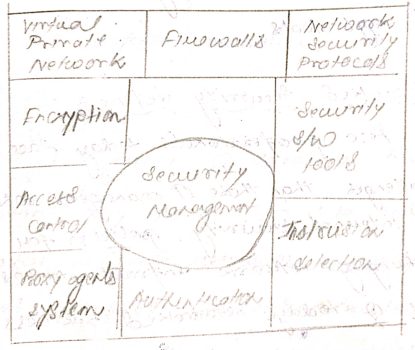
\includegraphics[width=0.48\textwidth]{secmeasure}
  \caption{Importance of security measures that are part of the
  security management of information system}
\end{figure}
\subsubsection{Data Backup}
The most critical type of data security measure. It is done by copying or
archiving data files. As a result, you can retrieve data in case of a data loss
event.

\subsubsection{Firewall}
A firewall is a network security system that monitors and controls incoming
and outgoing network traffic based on predetermined security rules. A
firewall typically establishes a barrier between a trusted network and an
untrusted network, such as the Internet.

\subsubsection{Encryption}
Encryption is the process of encoding information. This process converts the
original representation of the information, known as plain-text, into an
alternative form known as cipher-text. Ideally, only authorized parties can
decipher a cipher-text back to plain-text and access the original information.
Encryption does not itself prevent interference but denies the intelligible
content to a would-be interceptor.

\subsubsection{Security codes}
These are pre-assigned/generated codes that helps authenticate authorized 
personals.

\section{cybercrime}
cybercrime is the use of information technology for malicious activity. This 
can range from simply annoying computer users to huge financial loses and even
the loss of human life. With increase in the digitization of modern economy
and society, cybercrime has become a regular occurance.
\subsubsection*{Types of cybercrime:}
\begin{itemize}
  \item Identity theft.
  \item copyright Infringement.
  \item Click fraud.
  \item Advance fee fraud.
  \item Phising.
  \item Malware.
\end{itemize}

\section{Digital Signatures}
It is an electronic, encrypted, stamp of authentication on digital information
such as email, macros, electronic documents, etc. It confirms that the
information originated from the signer and has not been altered.
\begin{figure}[h]
  \centering
  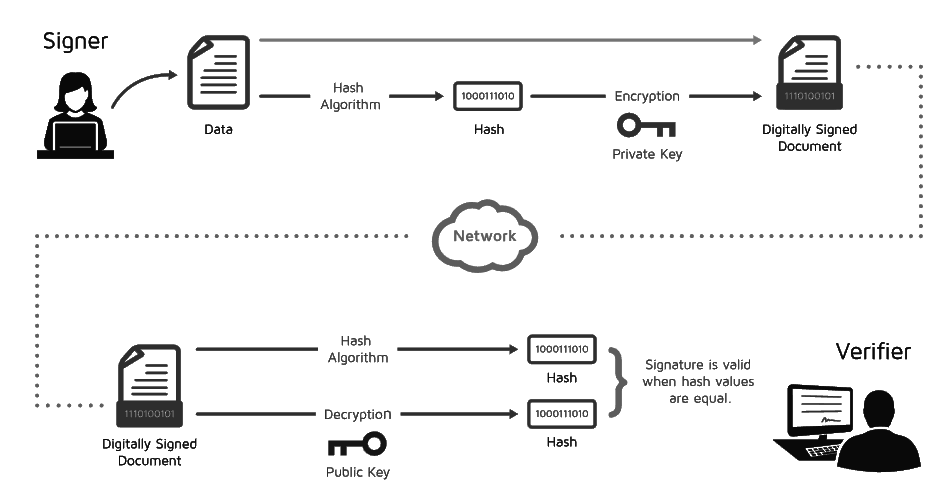
\includegraphics[width=0.5\textwidth]{key}
\end{figure}
\subsection{Advantages of digital signatures}
\begin{enumerate}
  \item Provides better security. Unauthorized person cannot do fraudulence in
    transactions.
  \item Helps you track the status of the documents on which the digital
    signature is applied.
  \item Businesses no longer have to wait for paper documents to be sent by
    courier. Contracts are easily written, completed, and signed by all
    concerned parties in a little amount of time no matter how far the parties
    are geographically.
  \item Signing an electronic document digitally identifies you as the
    signatory and that cannot be later denied.
  \item No one else can forge your digital signature or submit an electronic
    document falsely claiming it was signed by you.
\end{enumerate}

\subsection{Disadvantages of digital signatures}
\begin{enumerate}
  \item Digital signatures, like all technological products, are highly
    dependent on the technology it is based on. In this era of fast
    technological advancements, many of these tech products have a short shelf
    life.
  \item In order to effectively use digital signatures, both senders and
    recipients may have to buy digital certificates at a cost from trusted
    certification authorities.
  \item To work with digital certificates, senders and recipients have to buy 
    verification software at a cost.
  \item In some countries, laws regarding cyber and technology-based issues
    are weak or even non-existent. Trading in such jurisdictions becomes very
    risky for those who use digitally signed electronic documents.
  \item There are many different digital signature standards and most of them
    are incompatible with each other and this complicates the sharing of
    digitally signed documents.
\end{enumerate}

\section{Privacy issues of information management systems}
Privacy is an issue that concerns the computer community in connection with
maintaining personal information on individual citizens in computerized record
keeping systems.

Here are some of the most common issues faced by information management
systems:
\subsubsection{Embedding data privacy}
There is a broad lack of information and understanding about embedded
data, where it resides and the financial and reputational risk it posses
to businesses.
\subsubsection{Proliferating devices}
Data privacy becomes harder to handle when you factor in things like the
Internet of Things (IOT), bring-your-own-device IT policies and proliferating
internet-connected tablets, phones and watches.
\subsubsection{Increasing maintenance costs}
Keeping your systems secure and preventing data privacy issues at the
enterprise level can be expensive. But, the costs of a data breach are so
significant, you need to bite the bullet and invest properly.
\subsubsection{Access control is difficult in many industries}
Data privacy breaches are often caused by poorly managed access within an
organization. People and processes matter as much as technology. Humans are
the weakest link in the chain of privacy and security.
\subsubsection{Getting visibility into all of your data}
Using tools to discover and classify your data is essential. This will ensure
you can treat data uniquely and protect your sensitive data from any privacy
issues.
\subsubsection{A bad data culture}
Today, keeping data for its own sake broadens the attack surface for data
theft and increases the risk of breaching many data privacy laws.
Forward-thinking IT teams need to balance the value of collecting, storing and
processing large volumes of data against the pressing requirements for
privacy, security and compliance.
\subsubsection{Ever-increasing scale of data}
With hundreds of systems and millions of data records, we need a solution that
can handle the scale.

\section{How to prevent computer crime?}
\begin{center}
  \emph{(Major concerns about computer crime and privacy, and how to
  protect/prevent them.)}
\end{center}
There are different major concerns about computer crime and privacy on the
internet which refers to criminal conduct committed with the aid of a computer
or other electronic equipment connected to the internet.

Individuals or small groups with little technical knowledge and highly
organized worldwide criminal groups with relatively talented developers and 
specialists can engage in cybercrime.

\subsubsection{Stolen credit card information}
The most common cybercrime is when a person's credit card information is
stolen and used unlawfully to acquire or purchase goods or services over the
internet.
\subsubsection{Hacking government databases}
Another type of cybercrime is to tamper with sensitive government information
and data.
\subsubsection{Theft of user accounts}
Many website carrying peoples informations get breached on a regular basis 
nowadays. This results in extortion of user data on the dark web, and is sold 
to the highest bidder.
\subsubsection{Compromised IoT devices}
Most of the IoT devices are kept out of date with regards to their security 
updates, and due to the nature of these devices being connected to the
internet, hackers can get unauthorized access to devices and use those devices
for malicious activity.
\subsubsection{Loss of control and access to content:}
The WannaCry attack, which was allegedly launched by a state sponsored
criminal organization called `the lazurisk' from North-Korea, in 2017,
unleashed ransomware that locked-down thousands of computer mostly from the
NHS(\emph{National Health Security}) network, which are the government
hospitals across UK. Resulting in death of patients, delay in emergency
procedures and all other functions.

\section{How to protect our-self against cybercrime?}
\subsubsection{Use strong passwords}
Using a combination of alpha-numaric (abc123), special characters/symbols for a
password creates a hard to crack password. These tho are hard to crack are not
impossible to bypass, it just makes it difficult for anyone to just login to
your account without your permission.

It is also sometimes recommended to use a pass-phrase instead of a password 
due to the hard to guess nature of them.

\subsubsection{Regularly check of security updates}
Keeping softwares upto date is one of the most effective ways to protect a
device agains cyberattacks, these updates usually provide patches to bugs and 
newly discovered exploits and attacker can use to gain access to those devices.

\subsubsection{Keep most personal information off of social media}
This is one of most common yet the most easiest way to find information about
you is from your own social media, with all the digitization of society, every
one shares every single thing about their life, with inturn for someone seeking
to harm you is a goldmine, with these informations, they can do identity theft,
blackmail you, or do find any required informations.

To better protect against such threats, refrain from uploading everything you
do in real life.

\subsubsection{Secure your home network}
Using a local vpn will help you encrypt your unsecure plain \verb+http+ network
traffic into an \verb+https+ connection. This will make any kind of
man-in-the-middle attack impossible.

\subsubsection{Keep up with all major security breaches}
Being aware of all the major databreaches, cyberattacks will help you stay
vigilant and let you know when you need to change your passwords that could
have been breached on certain sites.




\newpage
\begin{tcolorbox}
  \part{Unit 5}
\end{tcolorbox}

\section{Procurement Management System}
Procurement management is responsible for overseeing all the processes involved
in acquiring the products, materials, goods and services needed for efficient
business operations. Depending on the business and industry, the terms
`sourcing,' `purchasing' and `procurement' may be used interchangeably to
describe the function of procuring supplies and managing the process, with
sourcing considered more strategic, and purchasing and procurement used to
refer to the actual operational function.

\subsection{Importance of Procurement?}
Without procurement, it would be impossible for most business operations to
function. Procurement management ensures that all items and services are
properly acquired so that projects and processes can proceed efficiently and
successfully.

\subsection{Steps of Procurement process}
\begin{itemize}
  \item Specifying and planning
  \item Identifying and selecting suppliers
  \item Negotiating and contracting
  \item Placing the purchase order
  \item Expediting
  \item Receipt and inspection of purchase
  \item Invoice clearing and payment
  \item Maintaining records and relationships
\end{itemize}

\section{ERP}
Enterprise resource planning (ERP) refers to a type of software that organizations use to manage day-to-day business activities such as accounting, procurement, project management, risk management and compliance, and supply chain operations. A complete ERP suite also includes enterprise performance management, software that helps plan, budget, predict, and report on an organization’s financial results.

e.g.:-ERP software for a manufacturing company will typically process the data from and track the status of sales invoicing as well as forecast raw material and HR requirement.

\subsection{Few example of ERP software}
Enterprise Resource Planning or in short ERP refers to the software that most of the businesses, right from the SMEs to enterprises use today for managing day-to-day business operations like accounting, project management, procurement, risk management, supply chain operations, manufacturing, sales and orders, managing customer relationships, human resources, finances, budgeting, reporting, and more. ERP systems are a suite of applications that work for different processes in a business, and stores all the data in a single centralised location, enabling easy transfer of data between the different areas of a business system. ERP software also automates these business activities and reduces time, and human efforts, thereby reducing delicacy of data at the same time.

Some of the amazing business benefits of using ERP software are improved and real-time data insights, low operational costs, enhanced collaboration, better efficiency of processes, elimination of data redundancy, etc.

\subsection{How ERP System works in an organizations like Amazon/Flipkart/Snapdeal?}

ERP systems work via a central database. Users look at dashboards to view real-time data across different business units such as sales, supply chain management, and personnel.
ERP is an integrated system of software applications that allows an organization to manage its business processes using a centralized relational database. It allows a business to see a snapshot of how efficiently its key functions, for example, inventory levels or sales, and personnel are working together.
ERP systems typically contain dashboards connected to a central database that let users look at real-time data across different business units.

\begin{figure}[ht]
  \centering
  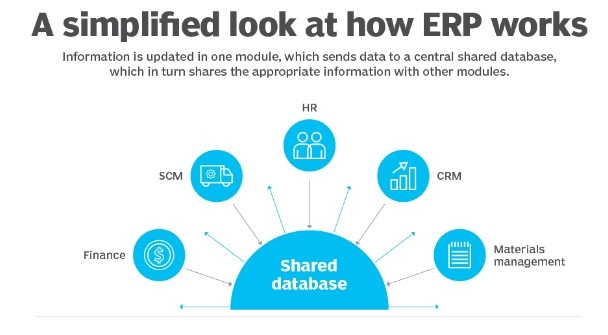
\includegraphics[width=\columnwidth]{howerpworks}
  \caption{A simplified look at how ERP works}
\end{figure}

In an ERP system, information is uploaded in one module and shared to the central database, which shares the information with other modules.

\subsubsection{Purchasing and procurement}
This module is for companies that require all their procurement and purchase activities streamlined, from vendor management to automatically routing approvals of payments and purchase order.

\subsubsection{HR}
This is a centralized digitized HR system that performs tasks from talent management to employee evaluating and tracking personnel hours.

\subsubsection{Finance}
This is a centralized system to track and record sales and operational information and payroll system and that has the ability to perform analysis reporting.

\subsubsection{Customer relationship management}
CRM enables a company to maintain a centralized repository of all the customers which can be accessed and utilized by all the customer oriented departments across the company.

\subsubsection{Business intelligence}
Business intelligence enables companies to view data analytics through dashboards metrics and pre-designed reports.

Amazon/Flipkart basically perform Online sales i.e  also known as e-commerce, the online sales module allows customers to see changes in prices, catalog, inventory and the supply chain, and have those changes reflected in customer-facing messaging. ERP vendors offer e-commerce applications for all sales channels, whether B2B, B2C or C2C. Ideally, this module allows us to manage both consumer and wholesale channels on a single platform. Online sales ERP applications can also let retail or wholesale partners update product information on their end.

\vskip10pt
\begin{figure}[h]
  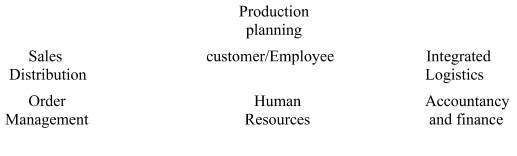
\includegraphics[width=\columnwidth]{majcomERP}
  \caption{Major application components of an ERP system}
\end{figure}

\section{Benefits and challenges of ERP}
\subsection{Quality and Efficiency}
ERP creates a framework for integrating and improving a companies internal business processes that results in significant improvements in the quality and efficiency of customer service production and distribution.

\subsection{Decision Support}
ERP provides vital cross functional information an business performance quickly to managers to significantly improve their ability to make better decisions in timely manner across the entire business enterprise.

\subsection{Enterprise agility}
Implementing ERP system breaks down many former departmental and functional walls of business process is and information resources. This result in most flexible organisational structures , managerial responsibilities and work roles and therefore a more agile and adaptive organisation and work force that can more easily capitalise or new business opportunities.

\subsection{Cost of ERP}
\resizebox{\columnwidth}{!}{
\begin{tabular}{ccc}
  & Hardware & \\
  & 12\% & \\
  Re-engineering & & Software \\
  43\% & & 15\%\\
  & & \\
  Data & & Training and\\
  Conversation & & chair management\\
  15\% & & 15\%\\
\end{tabular}}
\vskip10pt
An ERP implementation is like the corporate equivalent of a brain transplant. We pulled the plug on every company application and moved to people soft software. The risk was certainly disruption of business because if we do not do ERP properly we can kill our company guaranteed.


\section{Supply chain management (SCM)}
Starting an e-business takes ideas capital and technical user. Operating one, however, takes SCM skills. A successful SCM strategy is based on accurate order processing just in time inventory management and timely order fulfilment. SCM’s increasing importance illustrates how a tool that was a theoretical process ten years ago is now a hot competitive weapon. That’s why many companies today are making SCM a top strategic objective and major e-business application development initiative. Fundamentally SCM helps a company get the right products to the right place at the right time in proper quantity and an acceptable cost.

The goal of SCM is a cross functional enterprise system that uses it to helps support and manages the links between same of a compares key business process and low cost network of business relationships or supply chain to get a company’s products from concept to market.

\begin{figure}[ht]
  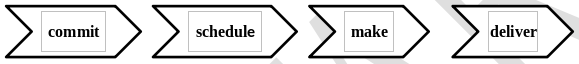
\includegraphics[width=\columnwidth]{scmlc}
  \caption{Supply chain life cycle}
\end{figure}

\begin{figure}[ht]
  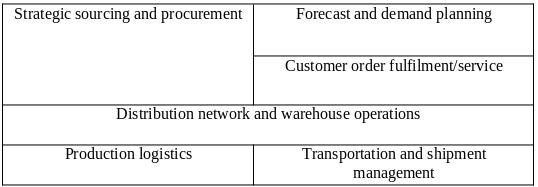
\includegraphics[width=\columnwidth]{scmfuncproc}
  \caption{SCM functional process}
\end{figure}


\section{Internet}
\begin{figure}[ht]
  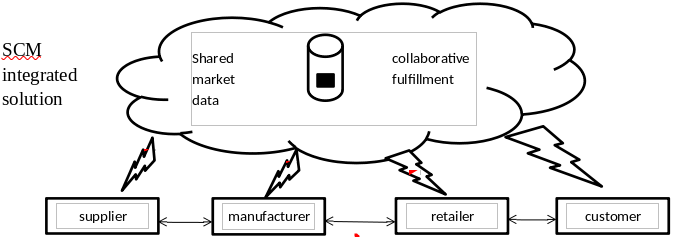
\includegraphics[width=\columnwidth]{scminter}
  \caption{Supply chain management}
\end{figure}
Software and internet technologies can help companies re-engineer and integrate the functional SCM process that support the supply chain life scale.

\subsection{Role of SCM}
The following figure helps us to understand the role and activities of supply chain management in business more clearly. The top there levels show the strategic tactical and operational objectives and outcomes of SCM  planning which are then accomplished by the business partners in a supply chain at the execution level of SCM.

\begin{figure}[ht]
  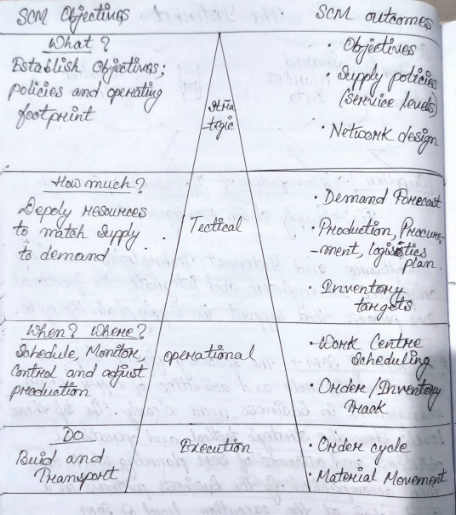
\includegraphics[width=\columnwidth]{roleofscm}
\end{figure}

\begin{figure}[ht]
  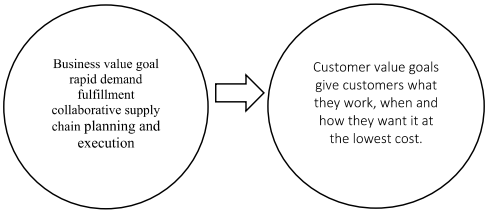
\includegraphics[width=\columnwidth]{objectivescm}
  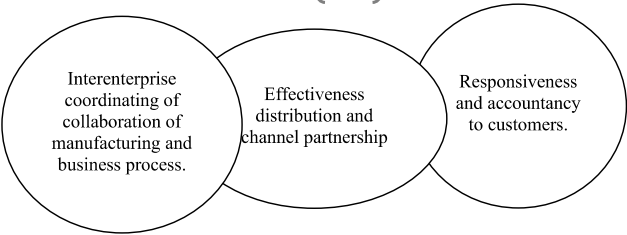
\includegraphics[width=\columnwidth]{objectivescm2}
  \caption{Objectives of SCM}
\end{figure}

\subsection{Stages in the use of supply chain management}
\begin{figure}[ht]
  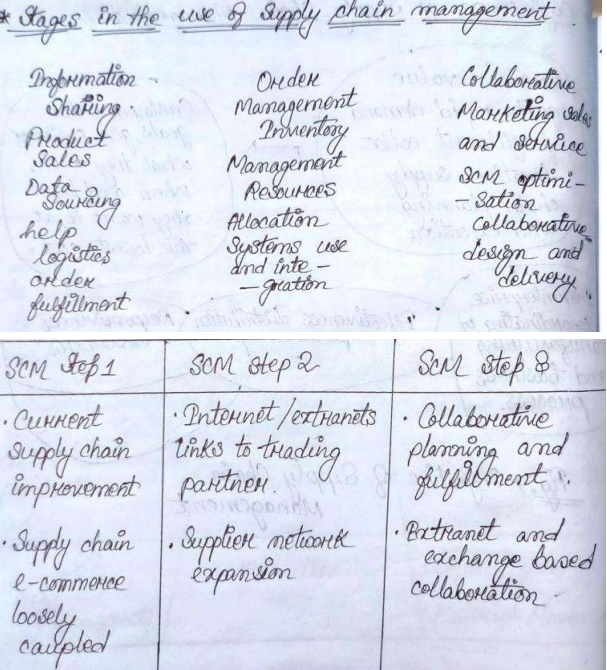
\includegraphics[width=\columnwidth]{stagesofscm}
\end{figure}

\section{Customer Relationship Management(CRM)}
Today customer in change. It is easier than ever for customer to comparism shop and with a click of the mouse to switch companies most valued asset. These relationships are worth more than the companies products, stores, factories, web address and even employees. Every companies strategy should address how to find and retail most profitable customers possible.

The primary business value of CR today is indisputable. Thus many companies are implementing CRM business initiatives and is part of a customer focused or customer centric strategy to improve their chances for success in todays competitive business environment.

\subsection{What is CRM?}
Managing the full range of customer relationship involves two related objectives:

One to provide the organization and all of its customer facing employees with a single complete view with every customer at every touch point an across all channels.
	
Two, to provide the customer with a single complete view of the company and its extended channels.

That’s why companies are turning to CRM to help then become customer-focused business CRM uses it to create a cross functional enterprise system that integrates and automates many of the customer serving process  in sales marketing and customer services that interact with a companies customer.

\subsection{Major application clusters in CRM}
CRM software helps sales marketing and service professionals capture and track relevant data about every past and plant contact with prospects and customer as well as other business and lifecycle events of customers. Information is captured from all customers touch point such as telephone, fax, e-mail the companies website, retail store and personal contact. CRM system store the data in a common  customer database that integrates all customer account information and makes it available throughout the company via internet , extranet or other network links for sales , marketing, service and other CRM application.

\begin{figure}[h]
  \centering
  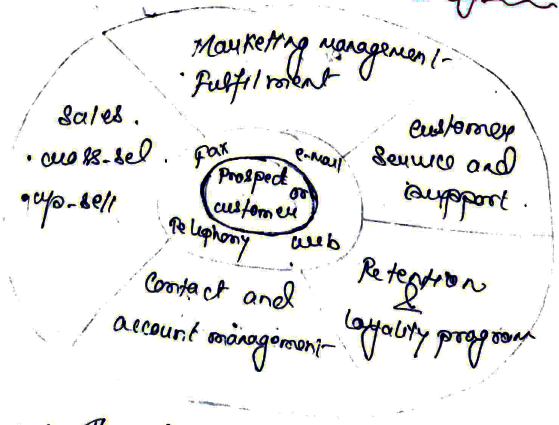
\includegraphics[width=0.47\textwidth]{CRMapplicationcluster}
  \caption{The major application clusters in CRM}
\end{figure}%}}}

\subsubsection{Roles}
CRM provides sales representation with the software tools and company data sources they need to support and manage their sales activities and optimize cross selling and up-selling. Examples includes sales prospect and product information product configuration and sales Grote generation  capabilities.

\subsubsection{Marketing}
CRM system help marketing professionals accomplish direct marketing campaigns by automating such task as qualifying leads for targeted marketing and scheduling and tracking direct marketing mailings. Then the CRM software helps marketing professionals capture and manage prospect and customer response data in the CRM database and analyse the customer and business value of a companies direct marketing campaigns.

\subsubsection{Customer service and support}
CRM system provides service with software tools and real time access to the common customer database shares by sales \& marketing professionals. CRM helps customer service managers create assign and manage requests for service by customers. Call centre software routes call to customer support agents based on their skills and authorities to handle specific kinds of service request help desk software assists customer services in helping customers who are having problems with a product or service by providing relevant service data and suggestions for resolving problems.

\subsubsection{Retention and loyalty programs}
\begin{itemize}
  \item It cost six times more to sell to a new customer than to sell to an existing one.
  \item A typical dissatisfied customer will tell eight to ten people about his/her experience.
  \item A company can boost its profits 85\% by increasing it sannual customer retention by only 5\%.
  \item The odds of selling a product to a new customer are 15\% where as the odds of selling product to an existing customer are 50\%.
\end{itemize}

That’s why enhancing and optimising customer retention and loyalty is a major business strategy and primary objective of relationship management. CRM system try to help a company identity, reward and market to their most loyal and profitable customers.

\subsection{Three phases of CRM}
We can view CRM as an integrated system of web enabled software tools and databases accomplishing a variety of customer focused business processes that support the three phases of the relations between a business and its customers.

\subsubsection{Acquire}
A business relies on CRM s/w tools and databases to help it acquire new customers by doing a superior job of  contact management ,sales prospecting ,selling ,direct marketing and fulfilment . The goal of these CRM functions is to help customers perceive the value of a superior product offered by an outstanding company.

\subsubsection{Enhance}
Web enabled CRM account management and customer service and support tools help keep customers happy by supporting superior service from a responsive network team of sales and service specialist and business partners. CRM sales force automation and direct marketing and fulfilment tools help companies cross-sell and up-sell to their customer thus increasing their profitability to their business.

\begin{figure}[ht]
  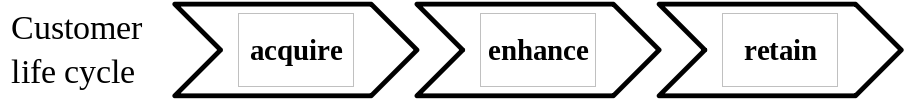
\includegraphics[width=\columnwidth]{cuslc}
\end{figure}

\begin{figure}[ht]
  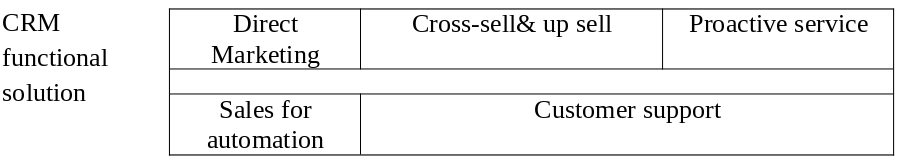
\includegraphics[width=\columnwidth]{crmfuncsol}
\end{figure}

\begin{figure}[ht]
  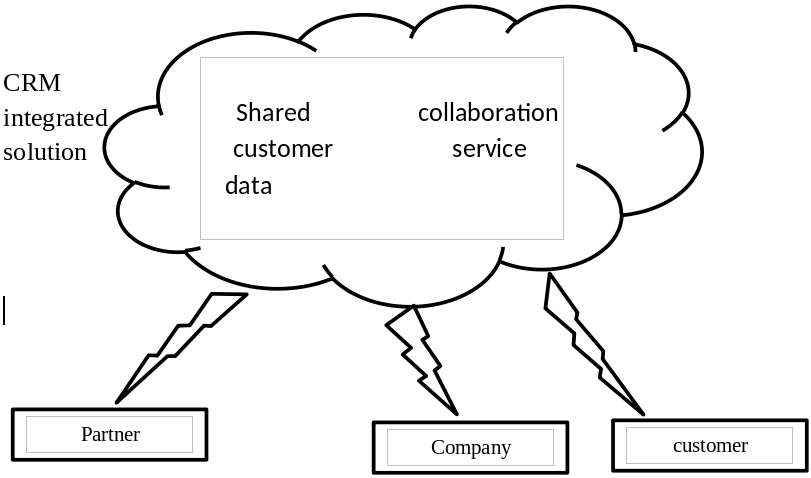
\includegraphics[width=\columnwidth]{crmintsol}
\end{figure}

\subsubsection{Retain}
CRM analytical software and database help company proactively identify and reward its most loyal and profitable customer to retain and expand their business via targeted marking and relationship marking programs. The value perceived by customers is of a rewarding personalized business relationship with them company.

\subsubsection{Benefits and challenges of CRM}
The potential business benefits of CRM are:

CRM allows a business to identify and target their best customers those who are the most profitable to the business , so they can be retained as life long customers for greater and more profitable services. It males possible real time customization and personalization of products and services  based on customer wants, needs etc. CRM can also keep track of when a customer contacts the company regardless of the contact point.


\end{document}
